% GENERATED by scripts/make_figure2.py. DO NOT EDIT BY HAND.
% Regenerate:
%   python3 scripts/make_figure2.py \
%     --out-tex paper/figures/fig2_before_after.tex \
%     --out-json paper/figures/fig2_values.json
%
% Requires \usepackage{tikz} and \usetikzlibrary{arrows.meta} in the preamble,
% both already loaded by paper/main.tex. No other package is needed.
%
% Provenance for every number here is paper/figures/fig2_values.json.
% SOURCE: paper/figures/fig1_values.json (accuracies, flip rates, churn, n,
%   and the 2,730 planning requirement, itself emitted from
%   scripts/audit_stats.py::required_n_for_tost by scripts/make_figure1.py)
% SOURCE: results/h3_eight_cell/paired_seeds_qwen25-7b_gsm8k.json
%   (joint_confidence_intervals.accuracy_delta, alpha, bootstrap_replicates)
% SOURCE: results/audit_verdicts_rev3.csv (eligible sources; margin_category;
%   v3_per_item_outputs), cross-checked against paper/audit_denominators.tex
% SOURCE: results/minigrid_run_20260722.manifest.json and
%   results/escalation_run_20260726.manifest.json (per-item cell JSONL count)
%
% TWO WORDINGS ARE LOAD-BEARING AND MUST NOT BE SOFTENED:
%   row 4 -- the required n is a PLANNING requirement at an assumed true
%     difference of zero. It says the evaluation cannot support the claim. It is
%     NOT evidence that the two methods differ.
%   row 2 -- no committed artifact records a TOST verdict for this cell. The
%     interval drawn is the committed 95% paired bootstrap interval, which is not
%     the 90% two-sided interval TOST at one-sided alpha=.05 requires, so it
%     decides nothing about the TOST either way.
\definecolor{fharm}{RGB}{140,45,20}
\definecolor{fben}{RGB}{125,178,219}
\definecolor{fneutral}{RGB}{110,110,110}
\definecolor{frule}{RGB}{60,60,60}

\begin{figure}[!t]
\centering
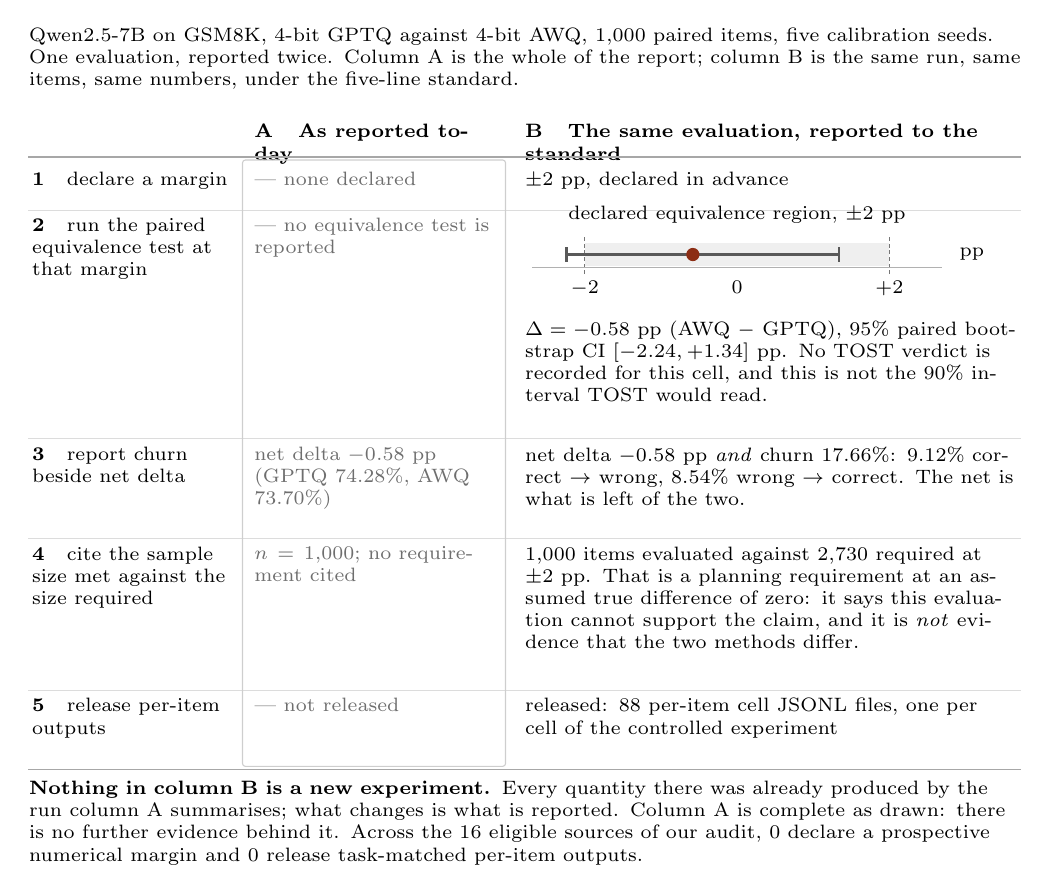
\begin{tikzpicture}[
  x=1cm, y=1cm, line width=0.5pt,
  font=\scriptsize,
  ttl/.style={font=\scriptsize\bfseries, anchor=north west},
  lbl/.style={font=\scriptsize, anchor=north west},
  gone/.style={font=\scriptsize, text=fneutral, anchor=north west},
]
\node[anchor=north west, inner sep=0, text width=12.6cm, font=\scriptsize] at (0,10.91) {Qwen2.5-7B on GSM8K, 4-bit GPTQ against 4-bit AWQ, $1{,}000$ paired items, five calibration seeds. One evaluation, reported twice. Column~A is the whole of the report; column~B is the same run, same items, same numbers, under the five-line standard.};
\node[ttl, text width=3.06cm, inner sep=0] at (2.86,9.68) {A\quad As reported today};
\node[ttl, text width=6.24cm, inner sep=0] at (6.3,9.68) {B\quad The same evaluation, reported to the standard};
\draw[frule!45, line width=0.5pt] (0,9.26) -- (12.6,9.26);
\node[lbl, text width=2.52cm, inner sep=0] at (0.04,9.08) {\textbf{1}\quad declare a margin};
\node[gone, text width=3.06cm, inner sep=0] at (2.86,9.08) {\textemdash\ none declared};
\node[lbl, text width=6.24cm, inner sep=0] at (6.3,9.08) {$\pm2$ pp, declared in advance};
\draw[frule!18, line width=0.3pt] (0,8.58) -- (12.6,8.58);
\node[lbl, text width=2.52cm, inner sep=0] at (0.04,8.49) {\textbf{2}\quad run the paired equivalence test at that margin};
\node[gone, text width=3.06cm, inner sep=0] at (2.86,8.49) {\textemdash\ no equivalence test is reported};
\draw[fill=frule!8, draw=none] (7.065,7.870) rectangle (10.935,8.170);
\draw[frule!70, line width=0.5pt, dash pattern=on 1.4pt off 1.0pt] (7.065,7.770) -- (7.065,8.270);
\draw[frule!70, line width=0.5pt, dash pattern=on 1.4pt off 1.0pt] (10.935,7.770) -- (10.935,8.270);
\node[font=\scriptsize, anchor=south] at (9.000,8.290) {declared equivalence region, $\pm2$ pp};
\draw[frule!40, line width=0.4pt] (6.400,7.850) -- (11.600,7.850);
\node[font=\scriptsize, anchor=north] at (7.065,7.810) {$-2$};
\node[font=\scriptsize, anchor=north] at (9.000,7.810) {$0$};
\node[font=\scriptsize, anchor=north] at (10.935,7.810) {$+2$};
\draw[frule!85, line width=0.9pt] (6.833,8.020) -- (10.296,8.020);
\draw[frule!85, line width=0.9pt] (6.833,7.930) -- (6.833,8.110);
\draw[frule!85, line width=0.9pt] (10.296,7.930) -- (10.296,8.110);
\draw[fill=fharm, draw=fharm] (8.439,8.020) circle (0.075);
\node[font=\scriptsize, anchor=west] at (11.700,8.020) {pp};
\node[lbl, text width=6.24cm, inner sep=0] at (6.3,7.19) {$\Delta = -0.58$ pp (AWQ $-$ GPTQ), 95\% paired bootstrap CI $[-2.24, +1.34]$ pp. No TOST verdict is recorded for this cell, and this is not the 90\% interval TOST would read.};
\draw[frule!18, line width=0.3pt] (0,5.68) -- (12.6,5.68);
\node[lbl, text width=2.52cm, inner sep=0] at (0.04,5.59) {\textbf{3}\quad report churn beside net delta};
\node[gone, text width=3.06cm, inner sep=0] at (2.86,5.59) {net delta $-0.58$ pp \\ (GPTQ 74.28\%, AWQ 73.70\%)};
\node[lbl, text width=6.24cm, inner sep=0] at (6.3,5.59) {net delta $-0.58$ pp \emph{and} churn 17.66\%: 9.12\% correct $\to$ wrong, 8.54\% wrong $\to$ correct. The net is what is left of the two.};
\draw[frule!18, line width=0.3pt] (0,4.41) -- (12.6,4.41);
\node[lbl, text width=2.52cm, inner sep=0] at (0.04,4.32) {\textbf{4}\quad cite the sample size met against the size required};
\node[gone, text width=3.06cm, inner sep=0] at (2.86,4.32) {$n = 1{,}000$; no requirement cited};
\node[lbl, text width=6.24cm, inner sep=0] at (6.3,4.32) {$1{,}000$ items evaluated against $2{,}730$ required at $\pm2$ pp. That is a planning requirement at an assumed true difference of zero: it says this evaluation cannot support the claim, and it is \emph{not} evidence that the two methods differ.};
\draw[frule!18, line width=0.3pt] (0,2.48) -- (12.6,2.48);
\node[lbl, text width=2.52cm, inner sep=0] at (0.04,2.39) {\textbf{5}\quad release per-item outputs};
\node[gone, text width=3.06cm, inner sep=0] at (2.86,2.39) {\textemdash\ not released};
\node[lbl, text width=6.24cm, inner sep=0] at (6.3,2.39) {released: 88 per-item cell JSONL files, one per cell of the controlled experiment};
\draw[frule!25, rounded corners=1pt, line width=0.4pt] (2.72,9.22) rectangle (6.0600000000000005,1.52);
\draw[frule!45, line width=0.5pt] (0,1.48) -- (12.6,1.48);
\node[anchor=north west, inner sep=0, text width=12.6cm, font=\scriptsize] at (0,1.34) {\textbf{Nothing in column~B is a new experiment.} Every quantity there was already produced by the run column~A summarises; what changes is what is reported. Column~A is complete as drawn: there is no further evidence behind it. Across the 16 eligible sources of our audit, 0 declare a prospective numerical margin and 0 release task-matched per-item outputs.};
\end{tikzpicture}
\caption{\textbf{The same evaluation, before and after the reporting standard.} Both columns describe one registered cell: Qwen2.5-7B on GSM8K, 4-bit GPTQ against 4-bit AWQ, $1{,}000$ paired items. \textbf{A}~is the aggregate report (two accuracies and a net delta of $0.58$~pp), and it is complete: there is no further evidence behind it. \textbf{B}~is the same run reported under the five lines of \S\ref{sec:conclusion}, and it needs no additional experiment. Row~2 draws the declared $\pm2$~pp margin together with the observed paired delta and the committed 95\% percentile-bootstrap interval for it; \emph{no TOST verdict exists for this cell}, and that interval is not the 90\% two-sided interval TOST at one-sided $\alpha=.05$ requires (\S\ref{sec:cert:method}), so it settles the equivalence question in neither direction. Row~4's $2{,}730$ is a \emph{planning} requirement computed at an assumed true difference of zero: it says this evaluation cannot support an equivalence claim at $\pm2$~pp, and it is not evidence that the two methods differ. Figure~\ref{fig:cancellation} decomposes the same cell; every value here is read from the artifacts recorded in \texttt{paper/figures/fig2\_values.json}.}
\label{fig:standard}
\end{figure}
